\documentclass[11pt]{article}

% Generic, journal-agnostic preamble. Before submission, replace this with the
% official Overleaf/LaTeX template for the target journal (e.g. SAGE's IJEEE
% class file) and re-flow these sections into it -- the content is written to
% be template-independent.

\usepackage[utf8]{inputenc}
\usepackage[T1]{fontenc}
\usepackage{graphicx}
\usepackage{amsmath}
\usepackage{amssymb}
\usepackage{booktabs}
\usepackage{hyperref}
\usepackage{tikz}
\usetikzlibrary{positioning, arrows.meta, fit, backgrounds}
\usepackage[margin=1in]{geometry}
\usepackage{caption}

\title{Mine Memristors: An Open-Source Minecraft Modification for Teaching\\
Analog Circuit Theory Through a Real Modified Nodal Analysis Solver}

\author{Rodrigo Picos\\
\small Universitat de les Illes Balears}

\date{}

\begin{document}
\maketitle

\begin{abstract}
We present Mine Memristors, an open-source modification (``mod'') for the sandbox game
Minecraft that turns the game world into an analog electronics laboratory. Players place
resistor, capacitor, inductor, and memristor blocks, wire them together with conductive
blocks, drive them with DC and time-varying sources, and probe the resulting voltages and
currents with a handheld oscilloscope, all rendered as ordinary game objects placed and
manipulated with the same mechanics used to build anything else in the game. Unlike
scripted or table-driven approximations of circuit behavior, every electrical quantity in
Mine Memristors is produced by a real modified nodal analysis (MNA) solver of the kind used
in SPICE-family simulators, including a charge-controlled linear-drift memristor model.
This paper describes the system's architecture, the circuit-theoretic design decisions
behind it (in particular, the explicit, player-placeable ground reference and the
topology-construction algorithm that keeps a component's own body from short-circuiting
itself), the pedagogical rationale for embedding a correct solver inside a game environment
rather than a dedicated simulator, and the verification methodology used during
development. We conclude with current limitations and a roadmap for classroom evaluation.
\end{abstract}

\section{Introduction}
\label{sec:introduction}

Teaching the transient and steady-state behavior of analog circuits is difficult precisely
because the phenomena involved -- charge accumulating on a capacitor plate, flux linking an
inductor's turns, a memristor's internal state drifting with the integral of the current
through it -- are invisible. Students are asked to reason about quantities they cannot see,
using differential equations whose solutions they are often meeting for the first time in
the same course. The traditional response is to pair the mathematics with a laboratory
bench and, increasingly, with software simulators such as SPICE~\cite{nagel1973spice},
LTspice, or browser-based tools such as the Falstad circuit simulator and PhET's Circuit
Construction Kit. These tools are effective, but they present the circuit as a schematic on
a two-dimensional canvas -- an abstraction one level removed from the physical act of
connecting components that a real breadboard or benchtop still preserves.

Sandbox games occupy an unusual middle ground. Minecraft in particular has an established
track record as an informal STEM learning environment, precisely because building something
inside it -- a redstone logic circuit, a working calculator, a piston-driven
elevator -- requires the same kind of systems thinking as an engineering task, while
remaining playful and low-stakes~\cite{nebel2016mining}. Minecraft's own redstone system is
already a widely used entry point into digital logic. There is, however, no equivalent for
\emph{analog} circuit theory inside the base game: redstone signals are effectively boolean,
propagated instantaneously (subject to a fixed per-block delay), with no notion of voltage,
current, capacitance, or continuous time.

This paper describes Mine Memristors, a modification (``mod'') for the Fabric mod loader
that adds a full set of analog circuit components to Minecraft: resistors, capacitors,
inductors, memristors, DC and time-varying voltage sources, an ammeter, wire, an explicit
ground reference block, and a handheld multi-channel oscilloscope probe. Placing and wiring
these blocks together builds a real circuit topology in the game world; a modified nodal
analysis solver, structurally the same technique used by SPICE-family
simulators~\cite{ho1975mna}, is re-solved every game tick (20~Hz) to drive every block's
displayed voltage, current, and internal state. Nothing in the mod is a scripted
approximation: an RC charging curve looks like an RC charging curve because the underlying
linear system is actually being solved, and a memristor's resistance drifts according to the
same charge-controlled ordinary differential equation used in the original HP linear-drift
model~\cite{strukov2008missing}, not a lookup table tuned to look plausible.

The remainder of this paper is organized as follows. Section~\ref{sec:related-work}
situates Mine Memristors relative to existing circuit simulators and the literature on
game-based engineering education. Section~\ref{sec:architecture} describes the mod's
software architecture, in particular the topology-construction algorithm used to translate
a player's in-world wiring into a circuit graph, and a subtle correctness bug in an earlier
version of that algorithm that is instructive in its own right.
Section~\ref{sec:circuit-solver} describes the solver itself, including the explicit,
player-placeable ground reference that lets the notion of ``ground'' be taught rather than
assumed. Section~\ref{sec:pedagogy} discusses the pedagogical rationale for each design
choice. Section~\ref{sec:validation} describes how the solver and the surrounding game logic
were verified during development. Section~\ref{sec:limitations} discusses current
limitations and planned classroom evaluation, and Section~\ref{sec:conclusion} concludes.

\section{Related Work}
\label{sec:related-work}

\subsection{Circuit simulators}

SPICE and its descendants~\cite{nagel1973spice} remain the reference implementation of
circuit simulation and are built around modified nodal analysis~\cite{ho1975mna}: node
voltages and a small number of auxiliary branch currents (one per independent voltage source
or inductor, in the classical formulation) are solved simultaneously at each timestep, with
reactive elements replaced by companion resistive/source models derived from a numerical
integration rule. Educational tools such as the Falstad circuit simulator and PhET's Circuit
Construction Kit lower the barrier to entry by replacing SPICE's netlist syntax with direct
schematic manipulation and are widely used in introductory courses. All three tools,
however, present the circuit as a two-dimensional schematic. CircuitCraft uses the same
underlying numerical technique (Sections~\ref{sec:architecture}
and~\ref{sec:circuit-solver} describe an MNA solver employing trapezoidal-integration
companion models for reactive elements, the family of technique SPICE itself uses) but
embeds it in a three-dimensional, first-person, block-based world rather than a schematic
canvas.

\subsection{Minecraft in education}
\label{sec:minecraft-in-education}

The instructional value of games and simulations has been studied extensively in general: a
meta-analysis by Sitzmann~\cite{sitzmann2011meta} found simulation games to be more
effective for training self-efficacy and knowledge retention than comparison instructional
methods across a range of technical domains. Minecraft occupies a disproportionately large
share of that broader literature. Microsoft maintains and markets a dedicated,
classroom-oriented variant of the game, \emph{Minecraft: Education Edition}, an indication of
how extensively the game had already been adopted informally by educators prior to this
commercial productization. Nebel et al.'s review~\cite{nebel2016mining} surveys this
literature broadly and identifies Minecraft's principal appeal for education as the same
property that makes it appealing as a game: an open, constructive world in which a learner's
own artifact, rather than a worked example, is the object of study, closely matching
Papert's constructionist framing~\cite{papert1980mindstorms}, discussed further in
Section~\ref{sec:pedagogy}.

Published case studies span a range of subjects well outside engineering. Bos et
al.~\cite{bos2014mathematics} describe using Minecraft to teach elementary-school
mathematics concepts, including area, perimeter, and ratio, through building tasks; Short's
account~\cite{short2012teaching} covers the use of the game to teach general science concepts
in a secondary-school setting; and Cipollone et al.~\cite{cipollone2014creative} present a
case study of Minecraft used as an open-ended creative tool, emphasizing collaboration and
planning skills rather than any specific curricular content. Callaghan's
survey~\cite{callaghan2016investigating} of Minecraft's role across primary and secondary
classrooms identifies a theme common to each of the studies above: teachers report high
engagement and motivation fairly consistently, whereas rigorously measured gains in specific
learning outcomes are reported less often and less consistently, a caveat also present in
the general simulation-games literature~\cite{sitzmann2011meta} and one this paper does not
claim to have resolved for CircuitCraft specifically (Section~\ref{sec:limitations}).

Within that broader literature, the subset closest to the present paper's subject concerns
Minecraft's native redstone subsystem, already a common entry point for teaching digital
logic and computer architecture concepts: players build logic gates, adders, and working
memory cells entirely from in-game blocks. Dezuanni et al.~\cite{dezuanni2015redstone}
document children describing and reasoning about redstone circuits in explicitly electrical
language, notwithstanding that the underlying mechanic is a discrete, boolean signal rather
than a continuous one (the mechanics of redstone itself are described in
Section~\ref{sec:minecraft-mechanics}). This is the literature to which CircuitCraft is
closest, and from which it departs most directly: the case studies cited above use
Minecraft's existing mechanics, redstone included, as the vehicle for a lesson, whereas Mine
Memristors introduces an entirely new, continuous-time simulation layer, because redstone's
discrete signal cannot represent voltage, current, or reactive state at all.

Beyond that academic literature, several existing Minecraft \emph{mods} -- as opposed to
case studies built on the base game -- add circuit-building mechanics of their own, and are
worth situating CircuitCraft against directly. Create: Circuits~\cite{chocoboyy2026createcircuits}
and ProjectRed~\cite{mrtjp2026projectred} both extend the redstone subsystem with more
compact logic-gate, arithmetic, and memory-latch blocks than vanilla redstone alone provides
-- ProjectRed as a modular suite (its Integration module specifically supplies the logic
gates, alongside separate modules for wiring, fabrication, and other redstone-adjacent
concerns). Create: Circuits labels some of its blocks (adder, multiplier, min, max) as
handling ``analog'' values, but only in the sense of Create's own multi-valued signal
strength, an integer quantity in the same fundamentally discrete sense as ordinary redstone
(Section~\ref{sec:minecraft-mechanics}), not a continuous electrical one; like ProjectRed, it
represents no voltage, current, or reactive state whatsoever, and both mods are purely
logical extensions of the same subsystem discussed above rather than a departure from it.
CircuitSim~\cite{dankov2026circuitsim} is, to the author's knowledge, the only prior
Minecraft mod that simulates genuinely analog circuits -- resistors, capacitors, inductors,
diodes, transistors, and op-amps among its components. It does so, however, by exporting a
player's in-world circuit as a netlist and invoking an external ngspice~\cite{nagel1973spice}
process, installed separately on the host system and on the system \texttt{PATH}, each time a
player right-clicks a dedicated ``simulate'' block, rather than solving the circuit natively
inside the mod itself. CircuitCraft's solver, by contrast, has no external dependency of any
kind, is embedded directly in the mod, and runs every game tick as an intrinsic part of the
running world -- driving the oscilloscope HUDs and the memristor's own evolving state live,
rather than producing a report a player consults after invoking a separate tool. To the
author's knowledge, it is the first Minecraft modification to embed a native, continuous-time
circuit solver for this purpose, rather than approximating one with the game's existing
discrete redstone mechanics or delegating it to an external simulator.

\subsection{Memristor theory and compact models}

The memristor was postulated on symmetry grounds by Chua~\cite{chua1971memristor} as a
fourth fundamental two-terminal circuit element, relating charge and flux, alongside the
resistor, capacitor, and inductor; a physical device exhibiting the predicted
charge-controlled behavior was subsequently reported by Strukov et al.\ at
HP~Labs~\cite{strukov2008missing}, whose linear-drift formulation is the model implemented
in this mod (Section~\ref{sec:circuit-solver}).

A substantial body of subsequent work refines or replaces this original formulation,
targeting shortcomings that only become apparent once the model is used for large-scale
circuit design or compared against fabricated devices. Biolek et
al.~\cite{biolek2009spice} introduce a window function that prevents the state variable
from becoming permanently pinned at either boundary during SPICE simulation, a numerical
issue that the original linear-drift formulation is otherwise prone to; Kvatinsky et
al.'s TEAM model~\cite{kvatinsky2013team} instead adopts a threshold-based switching
condition, trading some physical detail for a form that is considerably cheaper to simulate
at the scale of a large memristor-based circuit. Guan, Yu, and Wong~\cite{guan2012compact}
take a converse approach, developing a physics-based compact model of filament formation and
rupture, validated directly against measured resistive-switching device data, at the cost of
substantially greater model complexity. Picos et al.~\cite{picos2015chargeflux} formulate an
alternative approach that works directly in the charge--flux domain rather than through an
explicit resistance-state variable, and Al Chawa, Picos, and
Tetzlaff~\cite{alchawa2020simple} present a simplified compact model aimed specifically at
neuromorphic ReRAM applications, where computational efficiency across large device arrays
is often prioritized over matching any single device's measured characteristics exactly.

CircuitCraft implements Strukov et al.'s original linear-drift formulation specifically,
rather than any of the refinements above, because the priorities of a teaching tool differ
from those of a circuit designer or device physicist: the model must be simple enough to
verify in closed form (Section~\ref{sec:validation}) and traceable, step by step, to the
historically foundational definition a student is most likely to encounter first, rather
than optimized for matching a specific fabricated device's current--voltage characteristic
or for simulation efficiency across a large memristor array. Exposing one or more of the
alternative models above as a selectable preset -- in particular a windowed variant such as
Biolek et al.'s, which addresses a real limitation of the current implementation discussed
in Section~\ref{sec:limitations} -- is a natural extension of the present work.

\section{System Architecture}
\label{sec:architecture}

Mine Memristors is built on Fabric, a lightweight, widely used modding toolchain for
Minecraft. The codebase is organized into five packages, shown in
Figure~\ref{fig:architecture}: a solver package with no dependency on any Minecraft class at
all, a pair of packages describing the in-world blocks and their per-block simulation
state, a networking/topology package that ties placed blocks together into a circuit and
synchronizes probe readings to clients, and a client-only package responsible for rendering
the oscilloscope heads-up display.

\begin{figure}[htbp]
\centering
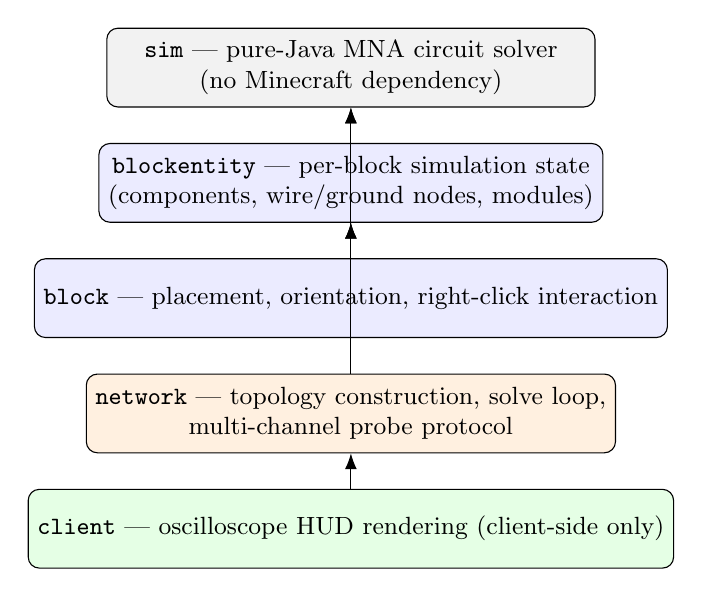
\begin{tikzpicture}[
    box/.style={draw, rounded corners, minimum width=6.2cm, minimum height=1cm,
                align=center, font=\small},
    node distance=0.45cm
]
\node[box, fill=gray!10] (sim) {\texttt{sim} --- pure-Java MNA circuit solver\\(no Minecraft dependency)};
\node[box, below=of sim, fill=blue!8] (blockentity) {\texttt{blockentity} --- per-block simulation state\\(components, wire/ground nodes, modules)};
\node[box, below=of blockentity, fill=blue!8] (block) {\texttt{block} --- placement, orientation, right-click interaction};
\node[box, below=of block, fill=orange!12] (network) {\texttt{network} --- topology construction, solve loop,\\multi-channel probe protocol};
\node[box, below=of network, fill=green!10] (client) {\texttt{client} --- oscilloscope HUD rendering (client-side only)};

\draw[-{Latex[length=2mm]}] (blockentity) -- (sim);
\draw[-{Latex[length=2mm]}] (block) -- (blockentity);
\draw[-{Latex[length=2mm]}] (network) -- (blockentity);
\draw[-{Latex[length=2mm]}] (network) -- (sim);
\draw[-{Latex[length=2mm]}] (client) -- (network);
\end{tikzpicture}
\caption{Package-level architecture. The solver has zero Minecraft dependencies and is
directly unit-testable with plain \texttt{javac}/\texttt{java}; every other layer builds on
it.}
\label{fig:architecture}
\end{figure}

\subsection{Components and topology}

Every two-terminal component (resistor, capacitor, inductor, memristor, the two voltage
sources, and an ammeter) occupies a single block, oriented along the horizontal or vertical
axis the player was facing when it was placed; its two electrical leads are its front and
back faces along that axis, and its other four faces are electrically insulated. A separate
wire block conducts on all six faces and has no orientation, and a ground block (see
Section~\ref{sec:circuit-solver}) behaves identically to wire for topology purposes.

Once per game tick, for each independent group of adjacent, mutually-conductive blocks
(a ``network''), the mod rebuilds a union--find partition over every block face that
presents a conductive surface toward a conductive neighbor, assigns one MNA node index to
each resulting partition, and asks every component in that network to stamp itself into the
circuit between its resolved node indices. Figure~\ref{fig:gallery} shows the full set of
component and utility blocks available to a player.

\begin{figure}[htbp]
\centering
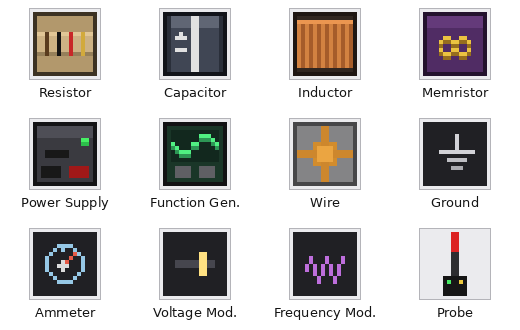
\includegraphics[width=0.85\textwidth]{figures/component_gallery.png}
\caption{The complete set of blocks and items provided by the mod.}
\label{fig:gallery}
\end{figure}

\subsection{A topology bug worth describing}
\label{sec:topology-bug}

An earlier version of the topology-construction algorithm keyed every participant in the
union--find structure by its block position alone, and unioned a component's own position
with each conductive neighbor in turn. For a plain wire block, conductive on all six faces
uniformly, this is correct: the block genuinely is a single electrical point, and merging it
with every conductive neighbor is exactly the desired behavior. For a two-terminal
component, however, this is wrong: unioning the component's position with its front
neighbor, and separately with its back neighbor, makes those two neighbors transitively
equivalent to one another \emph{through the component's own body}, because union--find
partitions are transitive. In other words, any component that had conducting material on
both of its leads simultaneously -- which is to say, any component actually wired into a
non-trivial circuit -- was silently short-circuited by the very algorithm meant to wire it
in, regardless of orientation or which component type it was. The fix, verified by
replaying a real in-world circuit's saved block data through both versions of the
algorithm offline, is to give a two-terminal component two independent partition
identities, one per lead, keyed by (position, side) rather than by the bare block position,
so that its two terminals can only be unified with one another by an actual external
connection, never by the component's own presence in the graph. Wire and ground blocks,
which are genuinely single electrical points, keep the simpler bare-position identity. This
episode is included here because it is a useful illustration for students in its own right:
a circuit topology bug that produces a mathematically singular system (a voltage source or
resistor with both terminals forced to the same node) is a natural, concrete example of why
a solver needs defensive numerical handling (Section~\ref{sec:circuit-solver}) even when the
graph-construction logic that feeds it is believed correct.

\subsection{Multi-channel oscilloscope protocol}

A handheld probe item lets a player pin up to three components, wires, or ground blocks at
once (right-click to pin or promote to most-recently-used, shift-right-click to unpin); the
server streams each pinned position's instantaneous voltage, current, a 200-sample rolling
history, and a short human-readable summary to that player once per tick, and the client
renders each of the up to three channels as an independently color-coded, auto-scaled
oscilloscope trace stacked in a corner of the screen. A component's trace shows the voltage
drop across its two leads (or, for the ammeter, the branch current, reusing the same
history/rendering machinery so that current and voltage can be watched side by side with no
separate ``current channel'' concept); a wire or ground block's trace shows its single
node's absolute voltage relative to whatever ground reference the network has, discussed
next.

\section{The Circuit Solver}
\label{sec:circuit-solver}

\subsection{Modified nodal analysis formulation}

The solver follows the standard MNA formulation~\cite{ho1975mna}. With $n$ non-ground nodes
and $m$ independent voltage sources, the unknown vector is the stacked node-voltage vector
$v \in \mathbb{R}^n$ and branch-current vector $j \in \mathbb{R}^m$ (one auxiliary unknown
per independent voltage source, the standard MNA treatment for an ideal source, which
cannot be described by a node-to-node conductance alone):
\begin{equation}
\begin{bmatrix} G & B \\ B^{\top} & 0 \end{bmatrix}
\begin{bmatrix} v \\ j \end{bmatrix}
=
\begin{bmatrix} i \\ e \end{bmatrix},
\end{equation}
where $G$ is the conductance matrix assembled by stamping every resistive (or
companion-resistive, see below) element, $B$ encodes which two nodes each voltage source is
connected across, $i$ collects any independent current injections, and $e$ is the vector of
source values at the current simulation time. Node~0 is reserved, by MNA convention, as the
ground reference and is excluded from the unknown vector entirely; every other node's
voltage is solved for relative to it. The resulting dense linear system is solved once per
game tick (every $1/20$~s of game time) by Gaussian elimination with partial pivoting.

To guard against a genuinely floating node -- a component with an unconnected lead, which a
player building a circuit incrementally will produce constantly and which must not crash
the simulation -- a small conductance ($10^{-9}$~S) is added to every non-ground node's
diagonal unconditionally. This is large enough to keep the matrix non-singular for an
isolated node, and small enough (roughly nine orders of magnitude below the smallest
resistor preset) to be numerically invisible in any circuit that is actually
connected.

\subsection{Reactive elements}

Capacitors and inductors are stamped using trapezoidal-integration companion models, the
same technique used in general-purpose circuit simulators, rather than backward Euler,
specifically because backward Euler introduces artificial numerical damping that would
visibly flatten an underdamped LC transient a student is trying to observe. For a capacitor
with capacitance $C$ and timestep $h$, the companion model is a conductance
$G_{eq} = 2C/h$ in parallel with a Norton current source
$I_{eq} = -G_{eq} v_C(t - h) - i_C(t-h)$, and correspondingly for an inductor,
$G_{eq} = h/(2L)$; both are re-derived from the trapezoidal rule
$x(t) \approx x(t-h) + \frac{h}{2}\left[\dot{x}(t) + \dot{x}(t-h)\right]$ applied to the
element's defining relation ($i = C\,\mathrm{d}v/\mathrm{d}t$ or
$v = L\,\mathrm{d}i/\mathrm{d}t$, respectively).

\subsection{The memristor}

The memristor implements Strukov et al.'s charge-controlled linear-drift
model~\cite{strukov2008missing}: its resistance is
\begin{equation}
R(q) = R_{on}\left(1 - \frac{q}{q_{max}}\right) + R_{off}\,\frac{q}{q_{max}}, \qquad
\dot{q}(t) = i(t),
\end{equation}
with $q/q_{max}$ clamped to $[0,1]$, defaults of $R_{on}=100\,\Omega$ and
$R_{off}=10\,000\,\Omega$, and a player-adjustable ``switching speed'' preset that scales
$q_{max}$. Because $q$ is the time-integral of the current actually flowing through the
device, its resistance depends on the device's entire history rather than its instantaneous
state -- the defining property that distinguishes a memristor from a resistor -- and,
notably, this state is deliberately preserved across a network topology rebuild
(Section~\ref{sec:limitations} discusses why the other reactive elements are not yet
afforded the same treatment).

\subsection{An explicit, player-placed ground reference}

MNA's ground node is, by construction, always present as a mathematical reference: node~0
is never actually solved for and is defined to be exactly $0$~V. Prior to the addition of a
dedicated ground block, however, nothing in the game world ever corresponded to node~0 --
every network's blocks were assigned freshly allocated node indices starting at~1, and
node~0 remained a purely internal bookkeeping device invisible to the player. This meant a
component's \emph{voltage drop} across its own two leads was always well defined (differences
between node voltages are invariant to which node is chosen as the reference), but there was
no way to ask a more basic question: ``what is the voltage \emph{at} this point in the
circuit?'', since that requires an agreed reference point, exactly as it does on a real
bench before a probe's ground clip is attached somewhere.

The ground block is conductive on all six faces, like wire, and is otherwise electrically
inert; the only special handling it receives is in the topology-construction step described
in Section~\ref{sec:architecture}, where any network partition containing a ground block is
assigned node index~0 directly instead of a freshly allocated index. No change to the
solver itself was required: the stamping routines already handled node~0 correctly
(a term referencing node~0 is simply omitted from the assembled matrix, per the standard
MNA convention), because it was always a valid destination for a component's terminal, just
never one a player could deliberately choose. Wire and ground blocks were, in the same
change, made directly probeable, so that a player can read the absolute voltage at any wired
point once a ground reference has been established elsewhere in the same network -- turning
the abstract idea of a reference node into something a player sets up explicitly, the same
way a real measurement requires choosing where to clip the ground lead before any other
reading is meaningful.

\subsection{Adjustable sources and value propagation}

The function generator's waveform shape (sine, square, or triangle) is a preset cycled
directly on the block, but its amplitude and frequency are set externally by two small
utility blocks -- a voltage module and a frequency module -- that a player places touching
the generator, or touching a chain of other modules of either kind that eventually reaches
one or more generators. Each module tracks two independently propagated quantities, a
voltage value and a frequency value, each tagged with the game tick at which it was last
\emph{authored} (set directly by a player right-clicking that specific module). A module
only authors the channel matching its own kind; for the other channel, it purely relays
whatever value and tag it last observed. Once per tick, every module compares both of its
channels against every immediately adjacent module of either kind and adopts whichever has
the more recent authoring tick, then pushes its resolved voltage and frequency to any
adjacent generator. This lets a single control reach an arbitrarily long, possibly mixed
chain of modules and every generator at its far end, converging one hop per tick (at
20 ticks/second, imperceptibly fast for any build a player is likely to construct), while
remaining simple enough to implement without a separate, explicit ``wiring'' concept distinct
from ordinary block adjacency.

\section{Pedagogical Design}
\label{sec:pedagogy}

The design choices described in Sections~\ref{sec:architecture}
and~\ref{sec:circuit-solver} were each made with a specific misconception or missing
intuition in mind, in the spirit of Papert's constructionism~\cite{papert1980mindstorms}:
a learner builds a working artifact and inspects its behavior directly, rather than being
shown the artifact's behavior secondhand.

\textbf{Wiring as physical placement, not schematic capture.} A component's two leads are
specific block faces, and two blocks are electrically connected only if each presents a
conductive face to the other. This is closer to breadboarding than to drawing a schematic:
a player who wires a resistor and a capacitor in what they intend to be a series loop, but
leaves a gap, gets a demonstrably incomplete circuit (Section~\ref{sec:circuit-solver}'s
floating-node handling means this fails safely rather than crashing), the same way a real
breadboard with a missing jumper simply does not work, rather than a schematic tool
flagging an unconnected pin as an abstract error.

\textbf{An explicit ground reference.} ``Voltage is always relative to a chosen reference''
is a standard remark in an introductory course, but it is easy for a student to receive it
as trivia rather than as something with consequences, because a schematic tool typically
draws a ground symbol for you, already connected, wherever the exercise needs it. Requiring
a player to place a ground block and wire it in themselves before a wire's absolute voltage
reading becomes meaningful (Section~\ref{sec:circuit-solver}) makes the reference an object
the player is responsible for, not a background assumption.

\textbf{Sources that must be switched on.} Both voltage sources are wired to a redstone
input and remain electrically inert -- an open circuit, contributing nothing to the solved
system -- until that input is active. This mirrors an actual laboratory workflow (wire the
circuit completely, verify it, \emph{then} switch the bench supply on) and, as a side
effect, is what makes the topology bug described in Section~\ref{sec:topology-bug} safe to
discuss with students directly: a source that is allowed to inject current into a circuit
whose leads are still both landing on the same node is not a hypothetical hazard invented
for this mod, it is the textbook definition of shorting a source across itself, and the fix
is the same for a player's bad wiring as it was for the mod's own construction algorithm.

\textbf{An oscilloscope that can watch more than one thing at once.} A single-channel
readout answers ``what is this component doing'', but the more interesting classroom
question is usually comparative -- how does the capacitor's voltage lag the source
driving it, or how does a resistor's voltage track a memristor's drifting resistance --
which requires watching multiple points simultaneously and comparing their phase and shape
against each other, not just their instantaneous values in isolation. Figure~\ref{fig:scope}
shows the in-game oscilloscope pinned to three points in the same circuit at once (a
function generator, a capacitor, and a resistor), reproducing the same relative-phase
comparison a real bench oscilloscope's multiple channels are used for.

\begin{figure}[htbp]
\centering
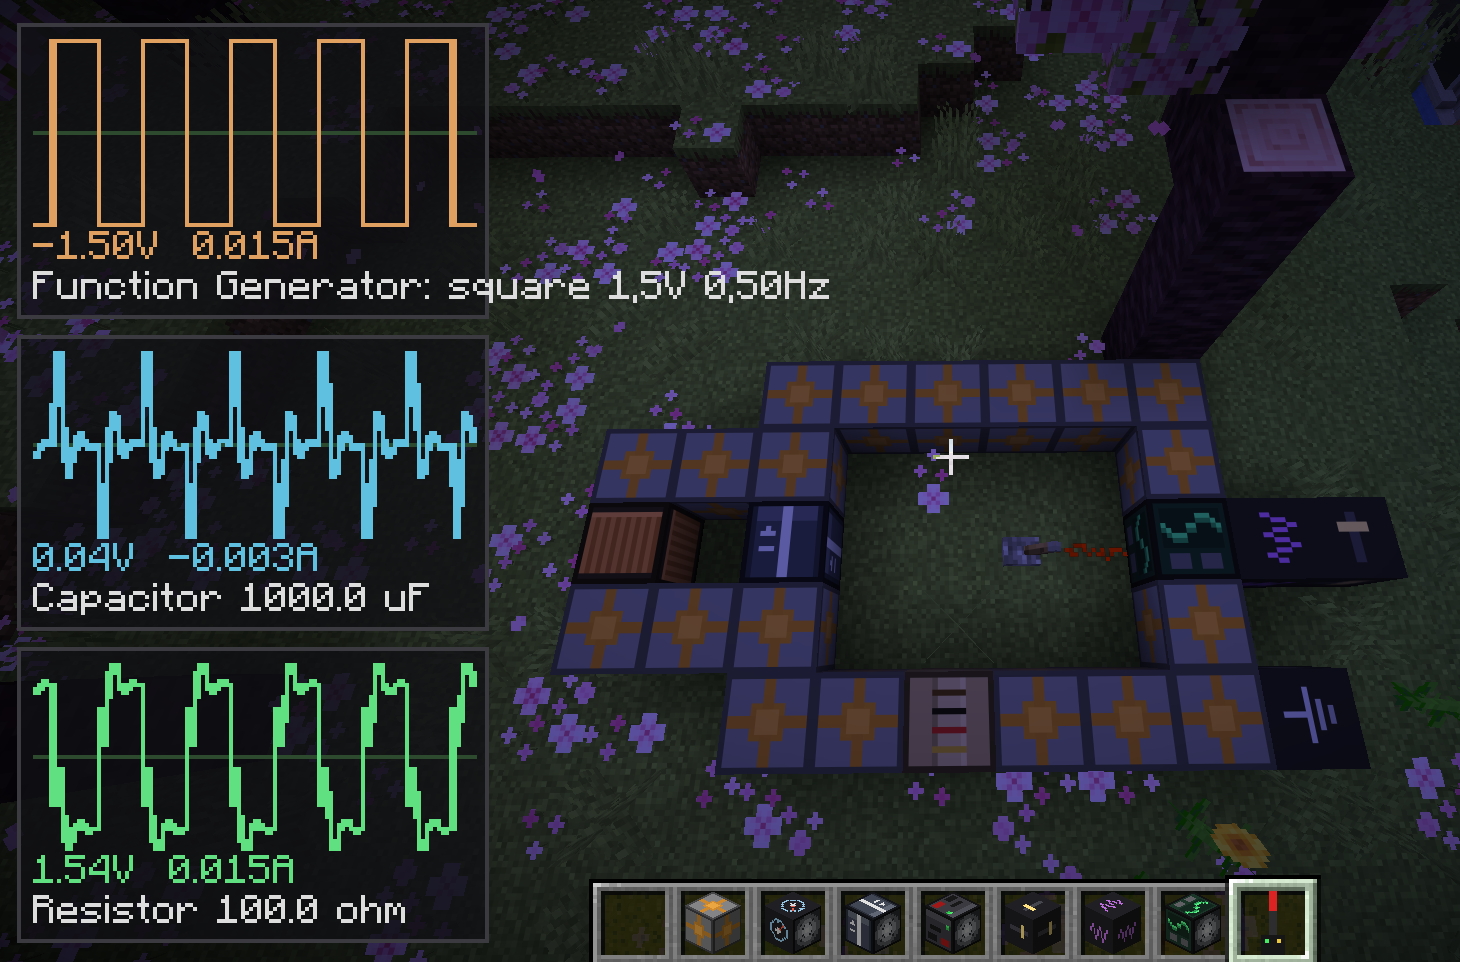
\includegraphics[width=0.48\textwidth]{figures/square_waveform.png}
\hfill
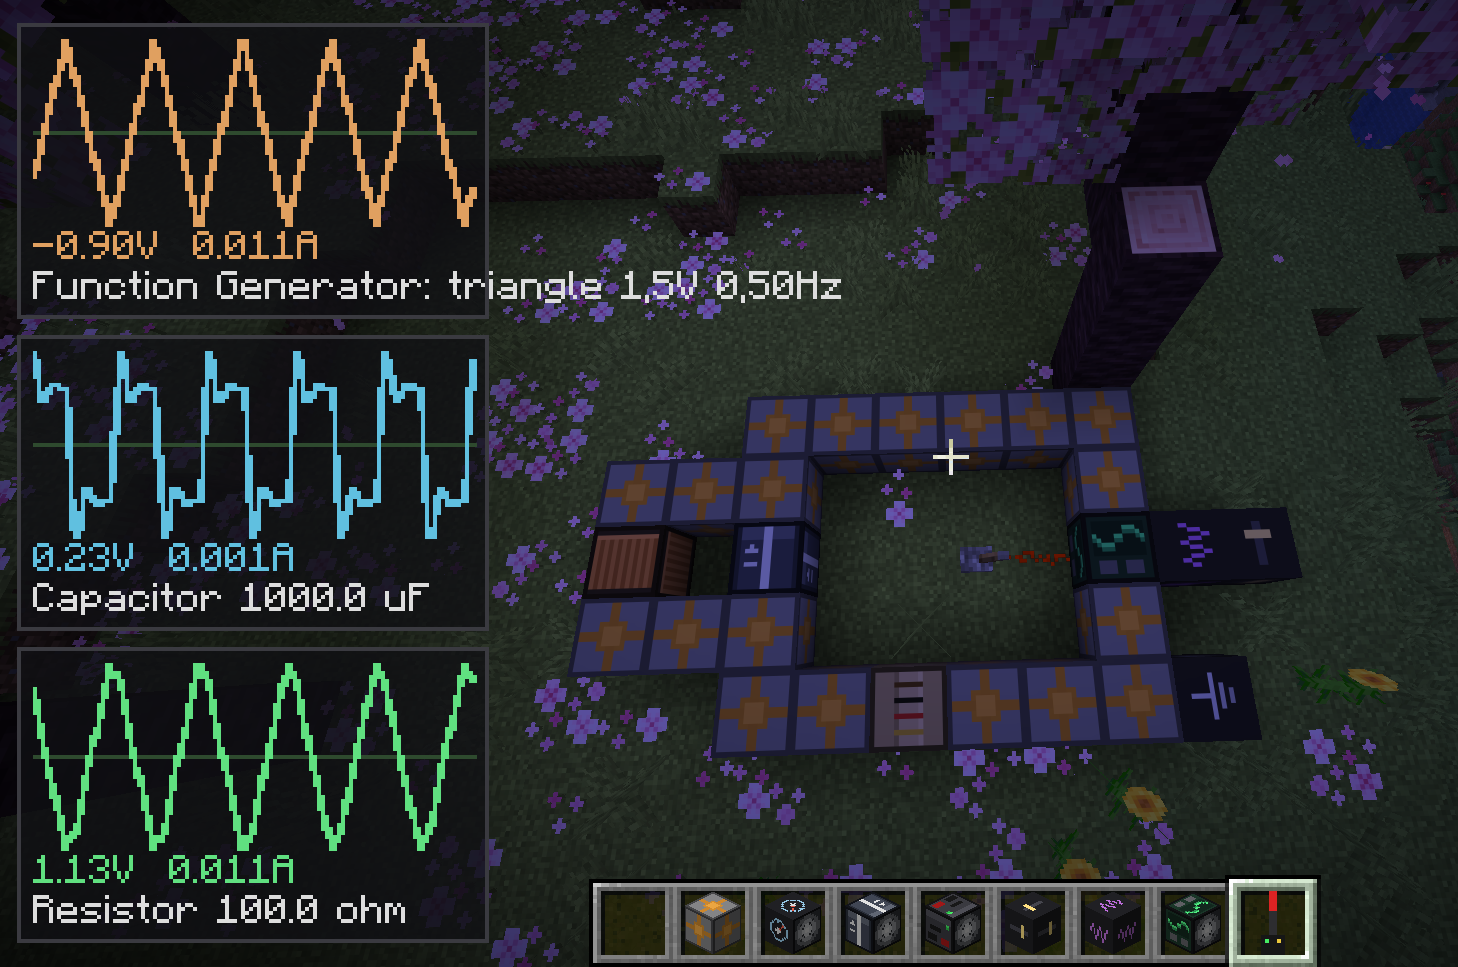
\includegraphics[width=0.48\textwidth]{figures/triangle_waveform.png}
\caption{The in-game multi-channel oscilloscope, pinned simultaneously to a function
generator (top trace), a capacitor (middle trace), and a resistor (bottom trace) in the same
circuit, driven by a square wave (left) and a triangle wave (right). Each trace is
independently auto-scaled and color-coded, with a live voltage/current readout and a summary
of that component's current state below its plot.}
\label{fig:scope}
\end{figure}

\section{Verification Methodology}
\label{sec:validation}

Because the entire point of the mod is that its behavior is not a scripted approximation,
each element's stamping and state-update routines were checked during development against
closed-form analytic solutions -- the exponential RC and RL step responses, and the
memristor's charge-controlled ODE integrated in closed form for a constant applied voltage
-- and agreed with those references to within approximately 1\%, consistent with the
timestep used (one Minecraft tick, $h = 1/20$~s) and the trapezoidal-integration companion
models' known truncation error. Because the solver package has no dependency on any
Minecraft class, this kind of check can be run as a plain Java program with no game
instance, decompiled game code, or build tooling involved, which made it practical to
re-check every element in isolation before wiring it into the rest of the mod.

The topology-construction bug described in Section~\ref{sec:topology-bug} was diagnosed and
confirmed using a different technique: rather than reasoning about the union--find algorithm
purely on paper, the actual block positions and orientations of a real, in-world circuit
were extracted directly from a saved world's region files and replayed offline, in a small
standalone script, through both the original and the corrected version of the algorithm.
The original algorithm collapsed the entire circuit to a single electrical node regardless
of the wiring's actual shape; the corrected version recovered the intended two-node series
loop. This is a useful diagnostic pattern in general when a bug is suspected in \emph{how a
game world is interpreted} rather than in a self-contained numerical routine: extracting the
authoritative world state and replaying the suspect logic against it offline is often more
conclusive than tracing the bug through the running game.

Because the mod targets a version of Minecraft (26.2) that predates the knowledge cutoff of
any large language model used to assist in its development, and that version introduced
several breaking changes to modding-relevant APIs (an unobfuscated mapping scheme, a
two-phase heads-up-display rendering interface, a redstone-neighbor-update signature change,
and a new per-item model-definition file format that a naively-written item registration
silently fails against), each such API surface was checked directly against the
decompiled game source and the mapped game jar for this specific version before being relied
upon, rather than against generic recollection of how equivalent APIs worked in earlier,
better-documented versions of the game. This is offered less as a claim specific to this mod
and more as a general observation for anyone building instructional software against a
platform that updates faster than the reference material describing it: verifying an
assumption against the authoritative source for the exact version in use is worth the extra
step whenever the platform is a moving target.

We note for transparency that, at the time of writing, this verification was performed
ad hoc during development rather than captured as a persisted, automatically re-run test
suite in the repository; formalizing the closed-form comparisons described above into a
checked-in regression suite is planned before a longer-term evaluation of the tool (see
Section~\ref{sec:limitations}), and would strengthen any reviewer's ability to independently
confirm the accuracy claims made here.

\section{Limitations and Future Work}
\label{sec:limitations}

\textbf{Reactive state resets on topology change.} The circuit for an entire network is
rebuilt from scratch whenever its wiring changes anywhere in that network, which resets a
capacitor's stored charge or an inductor's current to zero at that instant. The memristor is
deliberately exempted, since persistent state is its entire pedagogical point, but a student
who, e.g., extends a circuit while a capacitor is mid-charge will see that capacitor's
voltage reset rather than continue from where it was. Carrying reactive state across a
topology rebuild the same way the memristor's state is carried is planned future work and is
mostly a bookkeeping problem: the new topology's node indices must be matched back to the
element's previous node indices before its stored voltage or current can be meaningfully
re-applied.

\textbf{Fixed presets rather than continuous values.} Every adjustable quantity -- a
resistor's resistance, a source's amplitude or frequency -- is one of a small number of
discrete presets cycled by right-clicking, rather than a numeric entry. This keeps the
interaction model consistent with the rest of the base game (no custom text-entry GUI is
required) at the cost of the fine-grained control a real bench instrument offers; a
numeric-entry interface for these values is a natural extension.

\textbf{Solver scalability.} The MNA system for each independent network is solved by dense
Gaussian elimination every tick, which is adequate for the circuit sizes a single player
typically builds by hand, but scales as $O(n^3)$ in the number of independent nodes and does
not exploit the sparsity that a large circuit's conductance matrix would actually have. A
sparse solver, or amortizing re-solves across ticks when nothing electrically relevant has
changed, would be necessary before the tool could comfortably support very large
student-built circuits or a busy multiplayer server hosting many networks at once.

\textbf{Verification is currently informal.} As noted in Section~\ref{sec:validation}, the
closed-form comparisons used during development have not yet been captured as a persisted,
automatically re-run regression suite, and the tool's pedagogical effectiveness has so far
been assessed only informally by its author, not through a controlled classroom study. A
natural next step is a pre/post evaluation using an established circuits concept inventory,
comparing a cohort using Mine Memristors as a supplementary lab activity against a cohort
using a conventional schematic-based simulator, to test whether the game-based,
first-person construction experience described in Section~\ref{sec:pedagogy} produces a
measurable difference in conceptual understanding rather than only in engagement.

\textbf{Platform dependency.} The mod is necessarily tied to a specific version of
Minecraft and the Fabric mod loader, both of which are externally maintained and continue
to evolve; Section~\ref{sec:validation} discusses the verification discipline this
requires, but ongoing maintenance to track future game updates is an unavoidable cost of
building instructional software on top of an actively-developed commercial platform rather
than a purpose-built, stable simulator.

\section{Conclusion}
\label{sec:conclusion}

Mine Memristors embeds a real modified nodal analysis solver, complete with trapezoidal
reactive-element models and a charge-controlled memristor, inside an unmodified copy of
Minecraft's ordinary block-placing and wiring mechanics. Every voltage, current, and
internal component state a player observes is produced by actually solving the circuit the
player built, not by a scripted stand-in for one, down to details -- an explicit,
player-placed ground reference; sources that must be switched on before they contribute
current; a multi-channel oscilloscope that lets several points in the same circuit be
compared at once -- chosen specifically to make ideas that are usually assumed (a reference
node, a source being ``off'') into things a player must construct and reason about
themselves. The mod, its source, and this paper's typeset source are released under
permissive licenses; the authors welcome contributions, in particular toward the persisted
regression suite and the classroom evaluation described in
Section~\ref{sec:limitations}.


\bibliographystyle{plain}
\bibliography{references}

\end{document}
